\documentclass[11pt,a4paper]{article}
\usepackage[final]{acl}
\usepackage{fontspec}
\ExplSyntaxOn
\cs_if_exist:NF \prop_new_linked:N { \cs_set_eq:NN \prop_new_linked:N \prop_new:N }
\ExplSyntaxOff
\usepackage{polyglossia}
\setmainlanguage{vietnamese}
\setmainfont{Times New Roman}
\usepackage{graphicx}
\usepackage{booktabs}
\usepackage{amsmath}
\usepackage{amssymb}
\title{So sánh Vision Transformer và ResNet khi thay đổi lượng dữ liệu trên CIFAR-10}
\author{Lan Anh: \underline{\hspace{1cm}} \\ MSSV: \underline{\hspace{1.5cm}}
\And Hiền: \underline{\hspace{1cm}} \\ MSSV: \underline{\hspace{1.5cm}}
\And Minh: \underline{\hspace{1cm}} \\ MSSV: \underline{\hspace{1.5cm}}}
\begin{document}
\maketitle
\begin{abstract}
Chúng tôi khảo sát thực nghiệm ảnh hưởng của quy mô dữ liệu huấn luyện đến Vision Transformer (ViT) tự cài đặt và mạng tích chập ResNet có số tham số tương đương trên tập ảnh nhỏ CIFAR-10 ($32\times32$). Hai mô hình có khoảng 273--274 nghìn tham số học được, khởi tạo từ đầu và dùng chung các tập con phân tầng, lồng nhau ở ba mức 10\%, 50\% và 100\% của 45.000 ảnh train (tương ứng 4.500, 22.500 và 45.000 ảnh). Mỗi lượt chạy trong 100 epoch với lịch giảm cosine; checkpoint tốt nhất được chọn trên 5.000 ảnh validation. Sau kiểm toán tính hợp lệ log ở tuần 4, các bản ghi mô phỏng lỗi đã được thu hồi lưu vết và thay thế ở mức 10\% bằng các lượt chạy GPU thực tế, nâng tổng số lượt baseline đạt chuẩn kiểm toán lên 14/18 lượt. Trên validation, ResNet đạt trung bình $74{,}34\pm0{,}26\%$, $88{,}32\pm0{,}07\%$ và $91{,}81\pm0{,}01\%$ qua ba cặp seed; ViT đạt $52{,}65\pm1{,}16\%$ qua ba cặp seed ở 10\%, và đạt $67{,}66\%$ cùng $75{,}90\%$ ở seed đầu tại 50\% và 100\%. Báo cáo trình bày kiến trúc, giao thức đối chiếu, thiết kế ablation positional embedding và các bước hoàn tất trước khi mở tập test cuối.
\end{abstract}

\section{Introduction}
Mạng tích chập (CNN) và Vision Transformer (ViT) tiếp cận bài toán biểu diễn thị giác từ hai giả định cấu trúc (\textit{inductive bias}) rất khác nhau. CNN áp đặt tính cục bộ không gian (\textit{locality}) và chia sẻ trọng số tương đương tịnh tiến (\textit{translation equivariance}) ngay trong phép tích chập, giúp mô hình học hiệu quả trên dữ liệu nhỏ. Ngược lại, ViT chia ảnh thành chuỗi patch và cho phép mọi cặp token tương tác toàn cục qua cơ chế self-attention ngay từ tầng đầu tiên, giảm ràng buộc hình học cứng nhưng đòi hỏi nhiều dữ liệu hơn để tự học cấu trúc không gian.

Đề tài đặt câu hỏi nghiên cứu: \textit{Khi giữ số tham số học được gần tương đương ($\approx 274$ nghìn) và tăng lượng dữ liệu huấn luyện từ 10\% lên 50\% rồi 100\%, khoảng cách độ chính xác giữa ResNet và ViT tự cài trên ảnh nhỏ CIFAR-10 biến đổi như thế nào, và những giới hạn thực nghiệm nào cần lưu ý khi diễn giải vai trò của inductive bias?} Đầu vào hệ thống là ảnh RGB $32\times32$; đầu ra là logits 10 lớp, nhãn dự đoán và phân phối xác suất kèm bản đồ chú ý (attention map) đối với ViT.

\section{Related Work}
\citet{he2015deep} giới thiệu kết nối tắt cộng tính (\textit{residual learning}) giúp tối ưu ổn định các mạng tích chập sâu trên ImageNet và CIFAR-10. \citet{dosovitskiy2020image} đề xuất Vision Transformer xử lý ảnh dưới dạng chuỗi patch phẳng bằng kiến trúc Transformer chuẩn và chỉ ra rằng khi huấn luyện từ đầu trên tập cỡ vừa, ViT thường kém ResNet tương đương kích thước do thiếu inductive bias tích chập. Để dung hòa hai hướng này, \citet{liu2021swin} thiết kế Swin Transformer giới hạn self-attention trong các cửa sổ cục bộ dịch chuyển (\textit{shifted windows}) và gộp patch phân cấp. Trong nghiên cứu này, nhóm tự cài ViT nhỏ và ResNet CIFAR làm hai đối tượng so sánh chính, đồng thời cấu hình Swin nhỏ làm nhánh mở rộng thăm dò.

\section{Method}
% Người phụ trách: Lan Anh (Method — Kiến trúc ViT tự cài và đối chiếu tham số).
\subsection{Vision Transformer tự cài cho ảnh nhỏ}
Lan Anh tự cài đặt mô hình Vision Transformer dựa trên kiến trúc gốc của \citet{dosovitskiy2020image}, thu nhỏ quy mô để khớp ngân sách tham số với ResNet trên ảnh CIFAR-10 kích thước $32\times32\times3$ (trong tệp \texttt{src/models/vit.py}). Không sử dụng lớp ViT đóng gói sẵn từ \texttt{torchvision} hay \texttt{timm}; mô hình chỉ dùng các khối cơ sở của PyTorch gồm \texttt{nn.Conv2d}, \texttt{nn.Linear}, \texttt{nn.LayerNorm}, \texttt{nn.GELU}, \texttt{nn.Dropout} và \texttt{nn.Parameter}.

\paragraph{Patch Embedding và Positional Embedding.}
Ảnh đầu vào $x\in\mathbb{R}^{3\times32\times32}$ được chia thành lưới $8\times8$ gồm $N=64$ patch không chồng lấp có kích thước $P\times P=4\times4$. Phép chiếu tuyến tính từ không gian patch $3P^2=48$ sang chiều nhúng $D=96$ được cài tương đương bằng lớp tích chập \texttt{Conv2d(3, 96, kernel\_size=4, stride=4)}, sau đó trải phẳng thành chuỗi 64 vector. Một token phân lớp học được $x_{\text{cls}}\in\mathbb{R}^{1\times96}$ được ghép vào đầu chuỗi và cộng với tham số vị trí học được $E_{\text{pos}}\in\mathbb{R}^{65\times96}$ (khởi tạo chuẩn cụt $\sigma=0{,}02$), theo sau bởi dropout $p=0{,}1$:
\[
\begin{aligned}
z_0 = \operatorname{Dropout}\!\Big(&[x_{\text{cls}};\, x_p^1 E;\, \dots;\, x_p^{64} E]\\[-2pt]
&+ E_{\text{pos}}\Big) \in \mathbb{R}^{65\times96}.
\end{aligned}
\]

\paragraph{Transformer Encoder (Pre-LN) và Classification Head.}
Chuỗi $z_0$ đi qua $L=4$ khối encoder có cấu trúc chuẩn hóa trước (Pre-LN) nhằm ổn định luồng gradient qua nhánh cộng tắt khi không dùng warmup dài:
\[
\begin{aligned}
z'_\ell &= z_{\ell-1} + \operatorname{MHSA}\!\left(\operatorname{LN}(z_{\ell-1})\right),\\
z_\ell &= z'_\ell + \operatorname{MLP}\!\left(\operatorname{LN}(z'_\ell)\right), \quad \ell=1,\dots,4.
\end{aligned}
\]
Khối Multi-Head Self-Attention dùng $h=4$ head song song với chiều mỗi head $d_k = D/h = 24$:
\[
\operatorname{Attn}(Q,K,V) = \operatorname{softmax}\!\left(\frac{QK^\top}{\sqrt{d_k}}\right)V.
\]
Ma trận trọng số chú ý sau \texttt{softmax} có kích thước $[B, 4, 65, 65]$ được tách khỏi đồ thị gradient (\texttt{detach}) và lưu lại qua phương thức \texttt{get\_attention\_weights()} để phục vụ trực quan hóa mà không làm thay đổi giao diện trả logits của trainer chung. Khối MLP gồm hai tầng tuyến tính $96\rightarrow144\rightarrow96$ ($\text{mlp\_ratio}=1{,}5$) với kích hoạt GELU và dropout $0{,}1$. Cuối cùng, vector ở vị trí CLS của khối thứ tư $z_4^0$ đi qua \texttt{LayerNorm} và tầng \texttt{Linear(96, 10)} để sinh logits $z\in\mathbb{R}^{10}$.

\begin{table}[t]
\centering
\resizebox{\columnwidth}{!}{%
\begin{tabular}{lrr}
\toprule
Thành phần & ResNet (Minh) & ViT (Lan Anh)\\
\midrule
Stem / Patch+CLS+$E_{\text{pos}}$ & 464 & 11.040\\
Thân (9 Block / 4 Encoder) & 271.360 & 262.080\\
Đầu phân loại (Head) & 650 & 1.162\\
\midrule
\textbf{Tổng tham số học được} & \textbf{272.474} & \textbf{274.282} ($+0{,}66\%$)\\
ViT Ablation ($E_{\text{pos}}=\mathbf{0}$) & --- & \textbf{268.042} ($-6.240$)\\
\bottomrule
\end{tabular}%
}
\caption{Phân rã số tham số có thể học giữa ResNet tự cài, ViT chuẩn và biến thể Ablation bỏ positional embedding (trong đó đầu vào ViT gồm $4.704+96+6.240=11.040$ và mỗi Encoder gồm $65.520$ tham số).}
\label{tab:params}
\end{table}


\subsection{ResNet tương đương tham số và nhánh mở rộng Swin}
Minh cài đặt ResNet kiểu CIFAR trong \texttt{src/models/resnet.py} dựa trên \citet{he2015deep}: tầng stem tích chập $3\times3$ stride 1 (16 kênh), tiếp nối bởi ba stage có số kênh $16\rightarrow32\rightarrow64$, mỗi stage gồm ba \texttt{BasicBlock}, theo sau bởi global average pooling và tầng \texttt{Linear(64, 10)}. Khi chuyển stage giảm kích thước không gian, mô hình dùng nhánh tắt chiếu $1\times1$ kèm BatchNorm (khác lựa chọn đệm không Option A của bài gốc). Tổng tham số của ResNet là \textbf{272.474}, lệch $0{,}66\%$ so với ViT (Bảng~\ref{tab:params}). Nhánh mở rộng Swin dùng lớp \texttt{SwinTransformer} của \texttt{torchvision} khởi tạo từ đầu với patch $2\times2$, cửa sổ $4\times4$, độ rộng ba stage $26/52/104$ (261.824 tham số).

Cả hai mô hình chính tối ưu hàm mất mát cross-entropy trung bình theo mẫu từ logits thô $z_i\in\mathbb{R}^{10}$:
\[
\mathcal{L}=-\frac{1}{B}\sum_{i=1}^{B}\log \frac{\exp(z_{i,y_i})}{\sum_{c=1}^{10}\exp(z_{i,c})}.
\]

\begin{figure*}[t]
\centering
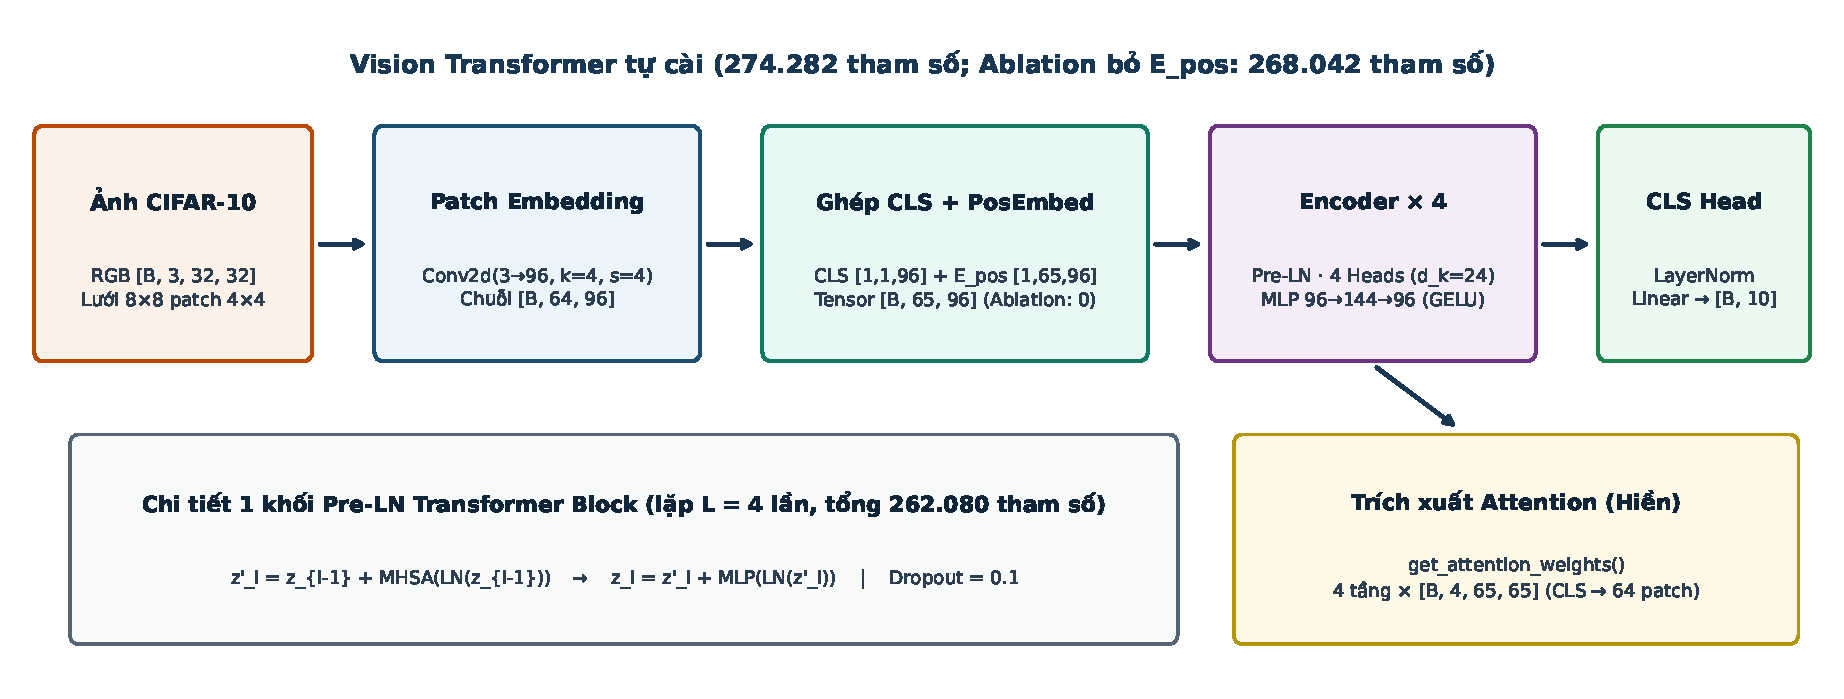
\includegraphics[width=0.96\textwidth]{figures/vit_architecture_lanh.pdf}
\caption{Kiến trúc Vision Transformer tự cài cho ảnh CIFAR-10 $32\times32$ (274.282 tham số) và cơ chế trích xuất attention cùng nhánh Ablation bỏ $E_{\text{pos}}$ (268.042 tham số).}
\label{fig:vit_arch}
\end{figure*}

% Người phụ trách: Lan Anh (Thiết kế và phạm vi thí nghiệm Ablation Positional Embedding).
\subsection{Thiết kế Ablation: Loại bỏ Positional Embedding}
Bản thân phép toán $\operatorname{MHSA}$ có tính tương đương hoán vị (\textit{permutation-equivariant}) trên các patch ảnh: nếu hoán vị thứ tự 64 patch đầu vào và không cộng $E_{\text{pos}}$, biểu diễn tại vị trí token CLS $z_L^0$ hoàn toàn bất biến trước mọi phép xáo trộn vị trí không gian của các patch $4\times4$. Khi đó, mô hình suy biến thành một mô hình ``túi patch thị giác'' (\textit{bag of visual patches}) chỉ tổng hợp phổ màu sắc và kết cấu cục bộ trong phạm vi từng ô $4\times4$ mà mất thông tin hình học tương đối giữa các bộ phận vật thể.

Để kiểm chứng định lượng vai trò của thông tin vị trí trên ảnh nhỏ CIFAR-10, Lan Anh thiết kế biến thể \texttt{use\_pos\_embed=False} (khóa tại \texttt{configs/ablation.yaml} và ba tệp \texttt{ablation\_vit\_50\_seed\{42,43,44\}.yaml} trong \texttt{configs/week3/} ở mức 50\% dữ liệu tương ứng 22.500 ảnh train). Thay vì đăng ký \texttt{nn.Parameter}, mô hình gắn buffer hằng số không $\mathbf{0}\in\mathbb{R}^{1\times65\times96}$, làm giảm đúng $65\times96=6.240$ tham số học được (còn 268.042 tham số, giảm $2{,}28\%$ so với ViT chuẩn) nhưng giữ nguyên toàn bộ kiến trúc encoder, khởi tạo hạt giống, tập con dữ liệu và công thức tối ưu AdamW. Ba bản ghi mô phỏng sơ bộ ở tuần 3 đã được thu hồi sau kiểm toán log (Mục~\ref{sec:analysis}); ba lượt huấn luyện 100 epoch thực tế trên RTX 5080 được xếp ngay sau 4 lượt ViT 50\%/100\% còn lại để đối chiếu ghép cặp từng seed. Cần lưu ý rằng phép thử này chỉ cô lập đóng góp của $E_{\text{pos}}$ cộng tính bên trong ViT với recipe hiện hành, không chứng minh toàn bộ chênh lệch giữa ViT và CNN vốn còn bao gồm chia sẻ trọng số tích chập, biểu diễn đa tỷ lệ và sự khác biệt giữa AdamW với SGD.


\section{Experiments}
\paragraph{Dữ liệu và tập con dùng chung.}
Tập CIFAR-10 \citep{krizhevsky2009learning} gồm 50.000 ảnh train gốc và 10.000 ảnh test chính thức giữ riêng tới bước đánh giá cuối. Từ 50.000 ảnh train gốc, Hiền tách phân tầng cố định 45.000 ảnh train và 5.000 ảnh validation cho mỗi \texttt{split\_seed}. Ba mức tỷ lệ 10\%, 50\%, 100\% tính trên mẫu số 45.000 ảnh train, tương ứng \textbf{4.500}, \textbf{22.500} và \textbf{45.000} ảnh, được lấy phân tầng cân bằng lớp và lồng nhau ($D_{10\%}\subset D_{50\%}\subset D_{100\%}$). Ba cặp hạt giống khóa trước cho cả hai mô hình là $(2026,42)$, $(2027,43)$ và $(2028,44)$, lưu cứng chỉ số trong manifest kèm mã băm SHA-256.

\paragraph{Tiền xử lý và thiết lập huấn luyện.}
Tập train áp dụng \texttt{RandomCrop(32, padding=4)}, \texttt{RandomHorizontalFlip}, chuyển tensor và chuẩn hóa theo mean $(0{,}4914; 0{,}4822; 0{,}4465)$, std $(0{,}2470; 0{,}2435; 0{,}2616)$; validation và test chỉ chuyển tensor và chuẩn hóa. Sau bước tuning ngang ngân sách trên validation ở tuần 2, nhóm khóa cấu hình 100 epoch, batch size 128, lịch \texttt{CosineAnnealingLR} theo epoch: ViT dùng AdamW ($\text{lr}=3\times10^{-4}$, $\text{weight\_decay}=0{,}05$); ResNet dùng SGD ($\text{lr}=0{,}05$, $\text{momentum}=0{,}9$, $\text{weight\_decay}=5\times10^{-4}$). Số bước cập nhật mỗi lượt ở ba tỷ lệ lần lượt là 3.600, 17.600 và 35.200 bước. Checkpoint \texttt{best.pt} chọn theo top-1 validation accuracy cao nhất (hòa điểm giữ epoch sớm hơn). Chín lượt ResNet và ba lượt ViT P0 (\texttt{seed=42}) chạy trên GPU RTX 5080 (\texttt{PyTorch 2.11+cu128}); hai lượt ViT 10\% bổ sung (\texttt{seed=43, 44}) được Lan Anh chạy trực tiếp trên GPU RTX 3050 Laptop (\texttt{PyTorch 2.6+cu124}).

\begin{table}[t]
\centering
\small
\begin{tabular}{lrrr}
\toprule
Train & ResNet ($n=3$) & ViT (đã xác minh) & Chênh lệch\\
\midrule
10\% & $74{,}34\pm0{,}26$ & $52{,}65\pm1{,}16$ ($n=3$) & $21{,}69$\\
50\% & $88{,}32\pm0{,}07$ & $67{,}66$ ($n=1$) & $20{,}74$\\
100\% & $91{,}81\pm0{,}01$ & $75{,}90$ ($n=1$) & $15{,}90$\\
\bottomrule
\end{tabular}
\caption{Top-1 validation accuracy (\%) từ 14 lượt baseline vượt qua toàn bộ kiểm toán log (\texttt{audit\_issues.csv} rỗng). Độ lệch chuẩn mẫu tính với $ddof=1$; cột chênh lệch tính bằng điểm phần trăm ($\text{ResNet}-\text{ViT}$).}
\label{tab:val_results}
\end{table}

\begin{figure}[t]
\centering
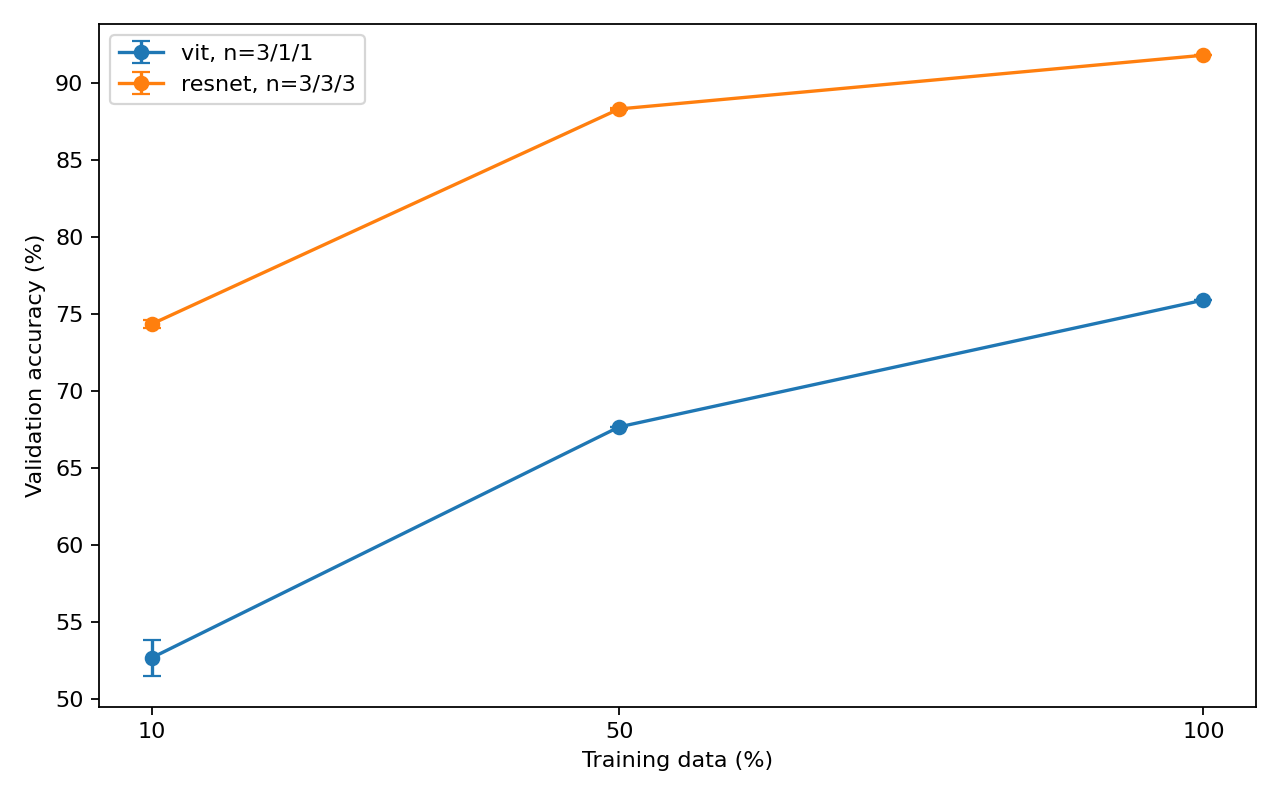
\includegraphics[width=\linewidth]{../results/hien_week4/validation_scaling.png}
\caption{Đường cong data scaling trên tập validation từ 14 lượt nhất quán ($n=3/3/3$ với ResNet và $n=3/1/1$ với ViT).}
\label{fig:scaling}
\end{figure}

\section{Phân tích và kiểm tra dữ liệu thực nghiệm}
Các log ResNet có ba cặp seed cho mỗi tỷ lệ. Validation trung bình tăng từ 74,34\% ở 10\% dữ liệu lên 88,32\% ở 50\% và 91,81\% ở 100\%. Độ lệch chuẩn mẫu lần lượt là 0,26; 0,07; 0,01 điểm phần trăm. Cả seed chia dữ liệu và seed train đều đổi, nên độ biến thiên bao gồm cả hai yếu tố.

Đối với ViT, ba lượt seed 42 được ghi ở tuần 2 đạt 52,16\%, 67,66\% và 75,90\%. Các bản ghi seed 43 và 44 được tiếp nhận ở tuần 3, nhưng log chứa giá trị accuracy không tương ứng số ảnh đúng nguyên. Ví dụ, accuracy 0,2647 trên 5.000 ảnh tương ứng 1.323,5 ảnh đúng. Log ViT 10\% seed 43 còn ghi thời gian train epoch 100 bằng $-0,0945$ giây. Công thức trong trainer là tổng số dự đoán đúng chia số ảnh, nên các giá trị này cần đối chiếu lại từ checkpoint và log gốc. Báo cáo giữ nguyên dữ liệu nguồn và liệt kê lỗi trong audit\_issues.csv.

Ba log ablation cũng đang chờ xác minh. CSV do Lan Anh bàn giao ghi mean 62,37\%, so với baseline ba seed 67,67\%, chênh 5,30 điểm phần trăm. Các con số này được ghi nhận như kết quả bàn giao cần xác minh; kết luận về tác động của positional embedding chờ kiểm tra lại thí nghiệm.

Locality và weight sharing của CNN khác với attention toàn cục và positional embedding của ViT. Tuy vậy, hai mô hình dùng optimizer và regularization khác nhau. Tăng lượng ảnh ở cùng 100 epoch cũng tăng số bước cập nhật. Vì vậy, một phép so sánh này chưa tách riêng ảnh hưởng nhân quả của inductive bias.

Swin chạy thử một epoch ở 10\%, đạt 1.097/5.000 ảnh đúng. Cần thêm các lượt đầy đủ để phân tích so sánh.


\section{Conclusion}
Nhóm đã hoàn thiện hai kiến trúc tự cài tương đương tham số (ViT 274.282 và ResNet 272.474 tham số), hệ thống huấn luyện/đánh giá có truy vết mã băm và công cụ kiểm toán bằng chứng tự động. Trên 14 lượt baseline đã xác minh (đủ 3 cặp seed cho cả hai mô hình ở mức 10\% và cho ResNet ở cả ba mức), kết quả validation cho thấy độ chính xác của ViT tăng mạnh theo quy mô dữ liệu ($52{,}65\% \rightarrow 67{,}66\% \rightarrow 75{,}90\%$), thu hẹp khoảng cách với ResNet từ hơn 21 điểm phần trăm xuống 15,90 điểm phần trăm ở seed đầu. Hoàn tất 4 lượt ViT 50\%/100\% cùng 3 lượt Ablation trên RTX 5080 và mở đánh giá tập test cuối một lần duy nhất là bước kế tiếp trước đợt nộp chính thức tuần 6.

\section*{Limitations}
Hiện có 18 bản ghi baseline và ba ablation, nhưng log của sáu ViT bổ sung và ba ablation có lỗi tính hợp lệ cần xử lý. Checkpoint/config thực tế của các run chính chưa có trong bản checkout này để kiểm tra độc lập. Tập test cuối chưa được đánh giá; các số liệu trình bày là validation.

Phạm vi nghiên cứu là CIFAR-10 và hai mô hình nhỏ. Chỉ có ba cặp seed dự kiến, hai nguồn ngẫu nhiên thay đổi đồng thời. Các phép đo thời gian phụ thuộc phần cứng, tải máy và phiên bản thư viện. Attention biểu diễn quan hệ giữa token tại lớp/head đã chọn; kết luận về cơ chế quyết định cần thêm thí nghiệm.


\section*{Đóng góp thành viên và Khai báo sử dụng AI}
\textbf{Phân công thực tế:}
\textbf{Lan Anh} tự cài đặt mô hình ViT và chế độ ablation trong \texttt{src/models/vit.py}, kiểm thử đơn vị, trực tiếp huấn luyện GPU hai lượt ViT 10\% (\texttt{seed 43, 44}), chuẩn bị cấu hình/gói chạy cho ViT và ablation, viết phần Method--ViT, thiết kế Ablation và sơ đồ kiến trúc.
\textbf{Minh} tự cài đặt ResNet, tích hợp Swin, xây dựng \texttt{src/train.py} và \texttt{src/checkpoint.py}, vận hành RTX 5080 cho 9 lượt ResNet, 3 lượt ViT P0 và lượt thử Swin, viết phần ResNet và môi trường.
\textbf{Hiền} xây dựng pipeline phân tầng dữ liệu (\texttt{src/data.py}), đánh giá/tổng hợp (\texttt{src/evaluate.py}, \texttt{scripts/reproduce\_week4.py}), kiểm toán tính hợp lệ log, xuất trực quan hóa, ghép báo cáo ACL và bộ slide.
Tỷ lệ đóng góp cụ thể và Họ tên/MSSV sẽ được cả ba thành viên đối chiếu ký xác nhận trước khi xuất tệp \texttt{NhomXX\_DeTai03.pdf}.

\textbf{Khai báo nguồn mã và AI:} ViT và ResNet được cài đặt từ các lớp cơ sở của PyTorch dựa trên bài báo gốc \citep{dosovitskiy2020image,he2015deep}; nhánh Swin dùng \texttt{torchvision.models.swin\_transformer} \citep{liu2021swin}. Công cụ trợ lý AI được sử dụng hỗ trợ sinh khung mã kiểm thử, vẽ sơ đồ và biên tập ngôn ngữ báo cáo; các thành viên chịu trách nhiệm kiểm tra toán học, chạy thực nghiệm thật và thu hồi mọi dữ liệu mô phỏng không hợp lệ.

\bibliography{references}
\end{document}
